\documentclass[twoside]{book}

% Packages required by doxygen
\usepackage{fixltx2e}
\usepackage{calc}
\usepackage{doxygen}
\usepackage[export]{adjustbox} % also loads graphicx
\usepackage{graphicx}
\usepackage[utf8]{inputenc}
\usepackage{makeidx}
\usepackage{multicol}
\usepackage{multirow}
\PassOptionsToPackage{warn}{textcomp}
\usepackage{textcomp}
\usepackage[nointegrals]{wasysym}
\usepackage[table]{xcolor}

% Font selection
\usepackage[T1]{fontenc}
\usepackage[scaled=.90]{helvet}
\usepackage{courier}
\usepackage{amssymb}
\usepackage{sectsty}
\renewcommand{\familydefault}{\sfdefault}
\allsectionsfont{%
  \fontseries{bc}\selectfont%
  \color{darkgray}%
}
\renewcommand{\DoxyLabelFont}{%
  \fontseries{bc}\selectfont%
  \color{darkgray}%
}
\newcommand{\+}{\discretionary{\mbox{\scriptsize$\hookleftarrow$}}{}{}}

% Page & text layout
\usepackage{geometry}
\geometry{%
  a4paper,%
  top=2.5cm,%
  bottom=2.5cm,%
  left=2.5cm,%
  right=2.5cm%
}
\tolerance=750
\hfuzz=15pt
\hbadness=750
\setlength{\emergencystretch}{15pt}
\setlength{\parindent}{0cm}
\setlength{\parskip}{3ex plus 2ex minus 2ex}
\makeatletter
\renewcommand{\paragraph}{%
  \@startsection{paragraph}{4}{0ex}{-1.0ex}{1.0ex}{%
    \normalfont\normalsize\bfseries\SS@parafont%
  }%
}
\renewcommand{\subparagraph}{%
  \@startsection{subparagraph}{5}{0ex}{-1.0ex}{1.0ex}{%
    \normalfont\normalsize\bfseries\SS@subparafont%
  }%
}
\makeatother

% Headers & footers
\usepackage{fancyhdr}
\pagestyle{fancyplain}
\fancyhead[LE]{\fancyplain{}{\bfseries\thepage}}
\fancyhead[CE]{\fancyplain{}{}}
\fancyhead[RE]{\fancyplain{}{\bfseries\leftmark}}
\fancyhead[LO]{\fancyplain{}{\bfseries\rightmark}}
\fancyhead[CO]{\fancyplain{}{}}
\fancyhead[RO]{\fancyplain{}{\bfseries\thepage}}
\fancyfoot[LE]{\fancyplain{}{}}
\fancyfoot[CE]{\fancyplain{}{}}
\fancyfoot[RE]{\fancyplain{}{\bfseries\scriptsize Generated by Doxygen }}
\fancyfoot[LO]{\fancyplain{}{\bfseries\scriptsize Generated by Doxygen }}
\fancyfoot[CO]{\fancyplain{}{}}
\fancyfoot[RO]{\fancyplain{}{}}
\renewcommand{\footrulewidth}{0.4pt}
\renewcommand{\chaptermark}[1]{%
  \markboth{#1}{}%
}
\renewcommand{\sectionmark}[1]{%
  \markright{\thesection\ #1}%
}

% Indices & bibliography
\usepackage{natbib}
\usepackage[titles]{tocloft}
\setcounter{tocdepth}{3}
\setcounter{secnumdepth}{5}
\makeindex

% Hyperlinks (required, but should be loaded last)
\usepackage{ifpdf}
\ifpdf
  \usepackage[pdftex,pagebackref=true]{hyperref}
\else
  \usepackage[ps2pdf,pagebackref=true]{hyperref}
\fi
\hypersetup{%
  colorlinks=true,%
  linkcolor=blue,%
  citecolor=blue,%
  unicode%
}

% Custom commands
\newcommand{\clearemptydoublepage}{%
  \newpage{\pagestyle{empty}\cleardoublepage}%
}

\usepackage{caption}
\captionsetup{labelsep=space,justification=centering,font={bf},singlelinecheck=off,skip=4pt,position=top}

%===== C O N T E N T S =====

\begin{document}

% Titlepage & ToC
\hypersetup{pageanchor=false,
             bookmarksnumbered=true,
             pdfencoding=unicode
            }
\pagenumbering{alph}
\begin{titlepage}
\vspace*{7cm}
\begin{center}%
{\Large Space Invaders }\\
\vspace*{1cm}
{\large Generated by Doxygen 1.8.13}\\
\end{center}
\end{titlepage}
\clearemptydoublepage
\pagenumbering{roman}
\tableofcontents
\clearemptydoublepage
\pagenumbering{arabic}
\hypersetup{pageanchor=true}

%--- Begin generated contents ---
\chapter{Hierarchical Index}
\section{Class Hierarchy}
This inheritance list is sorted roughly, but not completely, alphabetically\+:\begin{DoxyCompactList}
\item \contentsline{section}{util\+:\+:Clock}{\pageref{classutil_1_1Clock}}{}
\item \contentsline{section}{util\+:\+:Collision}{\pageref{classutil_1_1Collision}}{}
\item \contentsline{section}{entities\+:\+:Controller}{\pageref{classentities_1_1Controller}}{}
\begin{DoxyCompactList}
\item \contentsline{section}{entities\+:\+:enemies\+:\+:green\+\_\+alien\+:\+:Green\+Alien\+Controller}{\pageref{classentities_1_1enemies_1_1green__alien_1_1GreenAlienController}}{}
\item \contentsline{section}{entities\+:\+:enemies\+:\+:purple\+\_\+alien\+:\+:Purple\+Alien\+Controller}{\pageref{classentities_1_1enemies_1_1purple__alien_1_1PurpleAlienController}}{}
\item \contentsline{section}{entities\+:\+:enemies\+:\+:red\+\_\+alien\+:\+:Red\+Alien\+Controller}{\pageref{classentities_1_1enemies_1_1red__alien_1_1RedAlienController}}{}
\item \contentsline{section}{entities\+:\+:playership\+:\+:Player\+Ship\+Controller}{\pageref{classentities_1_1playership_1_1PlayerShipController}}{}
\item \contentsline{section}{entities\+:\+:projectiles\+:\+:standard\+:\+:Standard\+Projectile\+Controller}{\pageref{classentities_1_1projectiles_1_1standard_1_1StandardProjectileController}}{}
\item \contentsline{section}{entities\+:\+:projectiles\+:\+:standard\+\_\+enemy\+:\+:Standard\+Enemy\+Projectile\+Controller}{\pageref{classentities_1_1projectiles_1_1standard__enemy_1_1StandardEnemyProjectileController}}{}
\item \contentsline{section}{entities\+:\+:shield\+:\+:Shield\+Controller}{\pageref{classentities_1_1shield_1_1ShieldController}}{}
\end{DoxyCompactList}
\item enable\+\_\+shared\+\_\+from\+\_\+this\begin{DoxyCompactList}
\item \contentsline{section}{entities\+:\+:Observer}{\pageref{classentities_1_1Observer}}{}
\begin{DoxyCompactList}
\item \contentsline{section}{entities\+:\+:View}{\pageref{classentities_1_1View}}{}
\begin{DoxyCompactList}
\item \contentsline{section}{entities\+:\+:enemies\+:\+:green\+\_\+alien\+:\+:Green\+Alien\+View}{\pageref{classentities_1_1enemies_1_1green__alien_1_1GreenAlienView}}{}
\item \contentsline{section}{entities\+:\+:enemies\+:\+:purple\+\_\+alien\+:\+:Purple\+Alien\+View}{\pageref{classentities_1_1enemies_1_1purple__alien_1_1PurpleAlienView}}{}
\item \contentsline{section}{entities\+:\+:enemies\+:\+:red\+\_\+alien\+:\+:Red\+Alien\+View}{\pageref{classentities_1_1enemies_1_1red__alien_1_1RedAlienView}}{}
\item \contentsline{section}{entities\+:\+:playership\+:\+:Player\+Lives\+View}{\pageref{classentities_1_1playership_1_1PlayerLivesView}}{}
\item \contentsline{section}{entities\+:\+:playership\+:\+:Player\+Ship\+View}{\pageref{classentities_1_1playership_1_1PlayerShipView}}{}
\item \contentsline{section}{entities\+:\+:projectiles\+:\+:standard\+:\+:Standard\+Projectile\+View}{\pageref{classentities_1_1projectiles_1_1standard_1_1StandardProjectileView}}{}
\item \contentsline{section}{entities\+:\+:projectiles\+:\+:standard\+\_\+enemy\+:\+:Standard\+Enemy\+Projectile\+View}{\pageref{classentities_1_1projectiles_1_1standard__enemy_1_1StandardEnemyProjectileView}}{}
\item \contentsline{section}{entities\+:\+:shield\+:\+:Shield\+View}{\pageref{classentities_1_1shield_1_1ShieldView}}{}
\end{DoxyCompactList}
\item \contentsline{section}{World}{\pageref{classWorld}}{}
\end{DoxyCompactList}
\end{DoxyCompactList}
\item \contentsline{section}{Game}{\pageref{classGame}}{}
\item \contentsline{section}{entities\+:\+:projectiles\+:\+:Projectile\+Factory}{\pageref{classentities_1_1projectiles_1_1ProjectileFactory}}{}
\item \contentsline{section}{Space\+Settings}{\pageref{structSpaceSettings}}{}
\item \contentsline{section}{util\+:\+:Stopwatch}{\pageref{classutil_1_1Stopwatch}}{}
\item \contentsline{section}{entities\+:\+:Subject}{\pageref{classentities_1_1Subject}}{}
\begin{DoxyCompactList}
\item \contentsline{section}{entities\+:\+:Entity}{\pageref{classentities_1_1Entity}}{}
\begin{DoxyCompactList}
\item \contentsline{section}{entities\+:\+:enemies\+:\+:Enemy}{\pageref{classentities_1_1enemies_1_1Enemy}}{}
\begin{DoxyCompactList}
\item \contentsline{section}{entities\+:\+:enemies\+:\+:green\+\_\+alien\+:\+:Green\+Alien}{\pageref{classentities_1_1enemies_1_1green__alien_1_1GreenAlien}}{}
\item \contentsline{section}{entities\+:\+:enemies\+:\+:purple\+\_\+alien\+:\+:Purple\+Alien}{\pageref{classentities_1_1enemies_1_1purple__alien_1_1PurpleAlien}}{}
\item \contentsline{section}{entities\+:\+:enemies\+:\+:red\+\_\+alien\+:\+:Red\+Alien}{\pageref{classentities_1_1enemies_1_1red__alien_1_1RedAlien}}{}
\end{DoxyCompactList}
\item \contentsline{section}{entities\+:\+:playership\+:\+:Player\+Ship}{\pageref{classentities_1_1playership_1_1PlayerShip}}{}
\item \contentsline{section}{entities\+:\+:projectiles\+:\+:standard\+:\+:Standard\+Projectile}{\pageref{classentities_1_1projectiles_1_1standard_1_1StandardProjectile}}{}
\item \contentsline{section}{entities\+:\+:projectiles\+:\+:standard\+\_\+enemy\+:\+:Standard\+Enemy\+Projectile}{\pageref{classentities_1_1projectiles_1_1standard__enemy_1_1StandardEnemyProjectile}}{}
\item \contentsline{section}{entities\+:\+:shield\+:\+:Shield}{\pageref{classentities_1_1shield_1_1Shield}}{}
\end{DoxyCompactList}
\item \contentsline{section}{World}{\pageref{classWorld}}{}
\end{DoxyCompactList}
\item \contentsline{section}{util\+:\+:Transformation}{\pageref{classutil_1_1Transformation}}{}
\end{DoxyCompactList}

\chapter{Class Index}
\section{Class List}
Here are the classes, structs, unions and interfaces with brief descriptions\+:\begin{DoxyCompactList}
\item\contentsline{section}{\hyperlink{classutil_1_1Clock}{util\+::\+Clock} }{\pageref{classutil_1_1Clock}}{}
\item\contentsline{section}{\hyperlink{classutil_1_1Collision}{util\+::\+Collision} }{\pageref{classutil_1_1Collision}}{}
\item\contentsline{section}{\hyperlink{classobjects_1_1Controller}{objects\+::\+Controller} }{\pageref{classobjects_1_1Controller}}{}
\item\contentsline{section}{\hyperlink{classobjects_1_1enemies_1_1Enemy}{objects\+::enemies\+::\+Enemy} }{\pageref{classobjects_1_1enemies_1_1Enemy}}{}
\item\contentsline{section}{\hyperlink{classobjects_1_1enemies_1_1EnemyFactory}{objects\+::enemies\+::\+Enemy\+Factory} }{\pageref{classobjects_1_1enemies_1_1EnemyFactory}}{}
\item\contentsline{section}{\hyperlink{classobjects_1_1Entity}{objects\+::\+Entity} }{\pageref{classobjects_1_1Entity}}{}
\item\contentsline{section}{\hyperlink{classGame}{Game} }{\pageref{classGame}}{}
\item\contentsline{section}{\hyperlink{classobjects_1_1enemies_1_1green__alien_1_1GreenAlien}{objects\+::enemies\+::green\+\_\+alien\+::\+Green\+Alien} }{\pageref{classobjects_1_1enemies_1_1green__alien_1_1GreenAlien}}{}
\item\contentsline{section}{\hyperlink{classobjects_1_1enemies_1_1green__alien_1_1GreenAlienController}{objects\+::enemies\+::green\+\_\+alien\+::\+Green\+Alien\+Controller} }{\pageref{classobjects_1_1enemies_1_1green__alien_1_1GreenAlienController}}{}
\item\contentsline{section}{\hyperlink{classobjects_1_1enemies_1_1green__alien_1_1GreenAlienView}{objects\+::enemies\+::green\+\_\+alien\+::\+Green\+Alien\+View} }{\pageref{classobjects_1_1enemies_1_1green__alien_1_1GreenAlienView}}{}
\item\contentsline{section}{\hyperlink{classobjects_1_1Observer}{objects\+::\+Observer} }{\pageref{classobjects_1_1Observer}}{}
\item\contentsline{section}{\hyperlink{classobjects_1_1playership_1_1PlayerLivesView}{objects\+::playership\+::\+Player\+Lives\+View} }{\pageref{classobjects_1_1playership_1_1PlayerLivesView}}{}
\item\contentsline{section}{\hyperlink{classobjects_1_1playership_1_1PlayerShip}{objects\+::playership\+::\+Player\+Ship} }{\pageref{classobjects_1_1playership_1_1PlayerShip}}{}
\item\contentsline{section}{\hyperlink{classobjects_1_1playership_1_1PlayerShipController}{objects\+::playership\+::\+Player\+Ship\+Controller} }{\pageref{classobjects_1_1playership_1_1PlayerShipController}}{}
\item\contentsline{section}{\hyperlink{classobjects_1_1playership_1_1PlayerShipView}{objects\+::playership\+::\+Player\+Ship\+View} }{\pageref{classobjects_1_1playership_1_1PlayerShipView}}{}
\item\contentsline{section}{\hyperlink{classobjects_1_1projectiles_1_1ProjectileFactory}{objects\+::projectiles\+::\+Projectile\+Factory} }{\pageref{classobjects_1_1projectiles_1_1ProjectileFactory}}{}
\item\contentsline{section}{\hyperlink{classobjects_1_1enemies_1_1purple__alien_1_1PurpleAlien}{objects\+::enemies\+::purple\+\_\+alien\+::\+Purple\+Alien} }{\pageref{classobjects_1_1enemies_1_1purple__alien_1_1PurpleAlien}}{}
\item\contentsline{section}{\hyperlink{classobjects_1_1enemies_1_1purple__alien_1_1PurpleAlienController}{objects\+::enemies\+::purple\+\_\+alien\+::\+Purple\+Alien\+Controller} }{\pageref{classobjects_1_1enemies_1_1purple__alien_1_1PurpleAlienController}}{}
\item\contentsline{section}{\hyperlink{classobjects_1_1enemies_1_1purple__alien_1_1PurpleAlienView}{objects\+::enemies\+::purple\+\_\+alien\+::\+Purple\+Alien\+View} }{\pageref{classobjects_1_1enemies_1_1purple__alien_1_1PurpleAlienView}}{}
\item\contentsline{section}{\hyperlink{classobjects_1_1enemies_1_1red__alien_1_1RedAlien}{objects\+::enemies\+::red\+\_\+alien\+::\+Red\+Alien} }{\pageref{classobjects_1_1enemies_1_1red__alien_1_1RedAlien}}{}
\item\contentsline{section}{\hyperlink{classobjects_1_1enemies_1_1red__alien_1_1RedAlienController}{objects\+::enemies\+::red\+\_\+alien\+::\+Red\+Alien\+Controller} }{\pageref{classobjects_1_1enemies_1_1red__alien_1_1RedAlienController}}{}
\item\contentsline{section}{\hyperlink{classobjects_1_1enemies_1_1red__alien_1_1RedAlienView}{objects\+::enemies\+::red\+\_\+alien\+::\+Red\+Alien\+View} }{\pageref{classobjects_1_1enemies_1_1red__alien_1_1RedAlienView}}{}
\item\contentsline{section}{\hyperlink{classobjects_1_1shield_1_1Shield}{objects\+::shield\+::\+Shield} }{\pageref{classobjects_1_1shield_1_1Shield}}{}
\item\contentsline{section}{\hyperlink{classobjects_1_1shield_1_1ShieldController}{objects\+::shield\+::\+Shield\+Controller} }{\pageref{classobjects_1_1shield_1_1ShieldController}}{}
\item\contentsline{section}{\hyperlink{classobjects_1_1shield_1_1ShieldView}{objects\+::shield\+::\+Shield\+View} }{\pageref{classobjects_1_1shield_1_1ShieldView}}{}
\item\contentsline{section}{\hyperlink{classutil_1_1SpaceSettings}{util\+::\+Space\+Settings} }{\pageref{classutil_1_1SpaceSettings}}{}
\item\contentsline{section}{\hyperlink{classobjects_1_1projectiles_1_1standard__enemy_1_1StandardEnemyProjectile}{objects\+::projectiles\+::standard\+\_\+enemy\+::\+Standard\+Enemy\+Projectile} }{\pageref{classobjects_1_1projectiles_1_1standard__enemy_1_1StandardEnemyProjectile}}{}
\item\contentsline{section}{\hyperlink{classobjects_1_1projectiles_1_1standard__enemy_1_1StandardEnemyProjectileController}{objects\+::projectiles\+::standard\+\_\+enemy\+::\+Standard\+Enemy\+Projectile\+Controller} }{\pageref{classobjects_1_1projectiles_1_1standard__enemy_1_1StandardEnemyProjectileController}}{}
\item\contentsline{section}{\hyperlink{classobjects_1_1projectiles_1_1standard__enemy_1_1StandardEnemyProjectileView}{objects\+::projectiles\+::standard\+\_\+enemy\+::\+Standard\+Enemy\+Projectile\+View} }{\pageref{classobjects_1_1projectiles_1_1standard__enemy_1_1StandardEnemyProjectileView}}{}
\item\contentsline{section}{\hyperlink{classobjects_1_1projectiles_1_1standard_1_1StandardProjectile}{objects\+::projectiles\+::standard\+::\+Standard\+Projectile} }{\pageref{classobjects_1_1projectiles_1_1standard_1_1StandardProjectile}}{}
\item\contentsline{section}{\hyperlink{classobjects_1_1projectiles_1_1standard_1_1StandardProjectileController}{objects\+::projectiles\+::standard\+::\+Standard\+Projectile\+Controller} }{\pageref{classobjects_1_1projectiles_1_1standard_1_1StandardProjectileController}}{}
\item\contentsline{section}{\hyperlink{classobjects_1_1projectiles_1_1standard_1_1StandardProjectileView}{objects\+::projectiles\+::standard\+::\+Standard\+Projectile\+View} }{\pageref{classobjects_1_1projectiles_1_1standard_1_1StandardProjectileView}}{}
\item\contentsline{section}{\hyperlink{classutil_1_1Stopwatch}{util\+::\+Stopwatch} }{\pageref{classutil_1_1Stopwatch}}{}
\item\contentsline{section}{\hyperlink{classobjects_1_1Subject}{objects\+::\+Subject} }{\pageref{classobjects_1_1Subject}}{}
\item\contentsline{section}{\hyperlink{classutil_1_1Transformation}{util\+::\+Transformation} }{\pageref{classutil_1_1Transformation}}{}
\item\contentsline{section}{\hyperlink{classobjects_1_1View}{objects\+::\+View} }{\pageref{classobjects_1_1View}}{}
\item\contentsline{section}{\hyperlink{classWorld}{World} }{\pageref{classWorld}}{}
\end{DoxyCompactList}

\chapter{File Index}
\input{files}
\chapter{Class Documentation}
\input{classutil_1_1Clock}
\input{classutil_1_1Collision}
\input{classobjects_1_1Controller}
\input{classobjects_1_1enemies_1_1Enemy}
\input{classobjects_1_1enemies_1_1EnemyFactory}
\input{classobjects_1_1Entity}
\hypertarget{classGame}{}\section{Game Class Reference}
\label{classGame}\index{Game@{Game}}
\subsection*{Public Member Functions}
\begin{DoxyCompactItemize}
\item 
\hyperlink{classGame_ae84079995ee22675be0adfbaa54940d9}{Game} (const std\+::string \&settings)
\item 
void \hyperlink{classGame_a36587df95a3343658a2d02674050abd7}{play\+Levels} ()
\end{DoxyCompactItemize}


\subsection{Constructor \& Destructor Documentation}
\mbox{\Hypertarget{classGame_ae84079995ee22675be0adfbaa54940d9}\label{classGame_ae84079995ee22675be0adfbaa54940d9}} 
\index{Game@{Game}!Game@{Game}}
\index{Game@{Game}!Game@{Game}}
\subsubsection{\texorpdfstring{Game()}{Game()}}
{\footnotesize\ttfamily Game\+::\+Game (\begin{DoxyParamCaption}\item[{const std\+::string \&}]{settings }\end{DoxyParamCaption})\hspace{0.3cm}{\ttfamily [explicit]}}


\begin{DoxyParams}{Parameters}
{\em settings} & a json file containing the game settings \\
\hline
\end{DoxyParams}


\subsection{Member Function Documentation}
\mbox{\Hypertarget{classGame_a36587df95a3343658a2d02674050abd7}\label{classGame_a36587df95a3343658a2d02674050abd7}} 
\index{Game@{Game}!play\+Levels@{play\+Levels}}
\index{play\+Levels@{play\+Levels}!Game@{Game}}
\subsubsection{\texorpdfstring{play\+Levels()}{playLevels()}}
{\footnotesize\ttfamily void Game\+::play\+Levels (\begin{DoxyParamCaption}{ }\end{DoxyParamCaption})}

starts playing all the levels described in the settings file 

The documentation for this class was generated from the following files\+:\begin{DoxyCompactItemize}
\item 
/home/mano/\+Documents/univ/space\+\_\+invaders/src/game/\hyperlink{Game_8h}{Game.\+h}\item 
/home/mano/\+Documents/univ/space\+\_\+invaders/src/game/Game.\+cpp\item 
/home/mano/\+Documents/univ/space\+\_\+invaders/src/game/Game\+Screens.\+cpp\end{DoxyCompactItemize}

\input{classobjects_1_1enemies_1_1green__alien_1_1GreenAlien}
\input{classobjects_1_1enemies_1_1green__alien_1_1GreenAlienController}
\input{classobjects_1_1enemies_1_1green__alien_1_1GreenAlienView}
\input{classobjects_1_1Observer}
\input{classobjects_1_1playership_1_1PlayerLivesView}
\input{classobjects_1_1playership_1_1PlayerShip}
\input{classobjects_1_1playership_1_1PlayerShipController}
\input{classobjects_1_1playership_1_1PlayerShipView}
\input{classobjects_1_1projectiles_1_1ProjectileFactory}
\input{classobjects_1_1enemies_1_1purple__alien_1_1PurpleAlien}
\input{classobjects_1_1enemies_1_1purple__alien_1_1PurpleAlienController}
\input{classobjects_1_1enemies_1_1purple__alien_1_1PurpleAlienView}
\input{classobjects_1_1enemies_1_1red__alien_1_1RedAlien}
\input{classobjects_1_1enemies_1_1red__alien_1_1RedAlienController}
\input{classobjects_1_1enemies_1_1red__alien_1_1RedAlienView}
\input{classobjects_1_1shield_1_1Shield}
\input{classobjects_1_1shield_1_1ShieldController}
\input{classobjects_1_1shield_1_1ShieldView}
\input{classutil_1_1SpaceSettings}
\input{classobjects_1_1projectiles_1_1standard__enemy_1_1StandardEnemyProjectile}
\input{classobjects_1_1projectiles_1_1standard__enemy_1_1StandardEnemyProjectileController}
\input{classobjects_1_1projectiles_1_1standard__enemy_1_1StandardEnemyProjectileView}
\input{classobjects_1_1projectiles_1_1standard_1_1StandardProjectile}
\input{classobjects_1_1projectiles_1_1standard_1_1StandardProjectileController}
\input{classobjects_1_1projectiles_1_1standard_1_1StandardProjectileView}
\input{classutil_1_1Stopwatch}
\input{classobjects_1_1Subject}
\input{classutil_1_1Transformation}
\input{classobjects_1_1View}
\hypertarget{classWorld}{}\section{World Class Reference}
\label{classWorld}\index{World@{World}}


Inheritance diagram for World\+:
\nopagebreak
\begin{figure}[H]
\begin{center}
\leavevmode
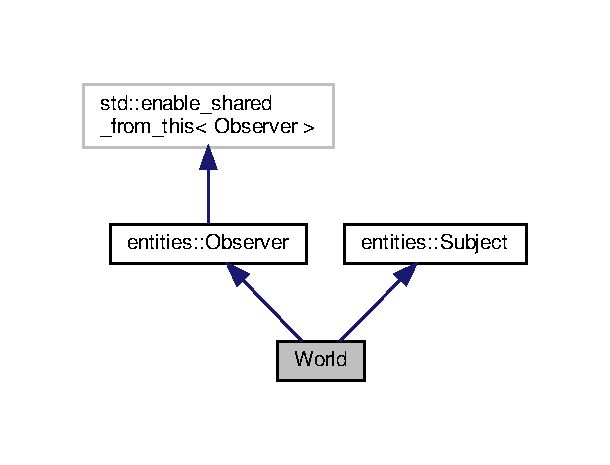
\includegraphics[width=200pt]{classWorld__inherit__graph}
\end{center}
\end{figure}


Collaboration diagram for World\+:
\nopagebreak
\begin{figure}[H]
\begin{center}
\leavevmode
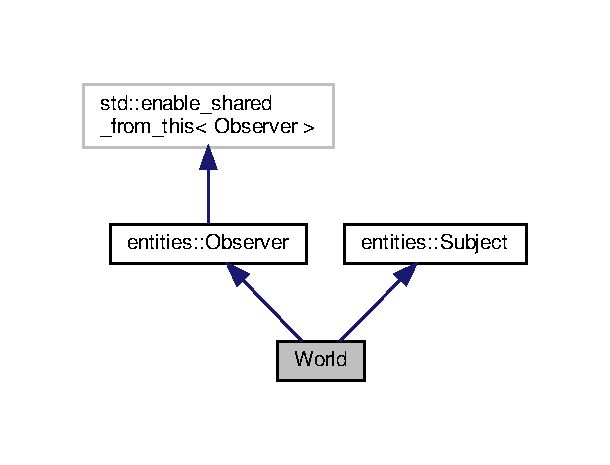
\includegraphics[width=200pt]{classWorld__coll__graph}
\end{center}
\end{figure}
\subsection*{Public Member Functions}
\begin{DoxyCompactItemize}
\item 
\hyperlink{classWorld_a96ca734b18df2cf85e666fc6d358e12c}{World} (std\+::shared\+\_\+ptr$<$ sf\+::\+Render\+Window $>$ window\+Ptr)
\item 
void \hyperlink{classWorld_a6a08c827c3a0def12b7700211353735f}{load\+Level} (const std\+::string \&filename)
\item 
void \hyperlink{classWorld_a91c2d7b127190f17a6cd85743245fb5b}{on\+Notify} () override
\item 
void \hyperlink{classWorld_ad37fe32cce284282361b9e7397b27a23}{handle\+Events} ()
\item 
void \hyperlink{classWorld_a5cc73b1aa54db5da01e4004acd4fd8bb}{update\+Entities} ()
\item 
void \hyperlink{classWorld_a8e8ad60668f8fe975f03bcb612264bc4}{draw\+Views} ()
\item 
void \hyperlink{classWorld_a04f39f13be0b568122bc8a539c15f014}{enter\+Endless} ()
\item 
\mbox{\Hypertarget{classWorld_a89826be651c0ea4c8965403cd0b8138c}\label{classWorld_a89826be651c0ea4c8965403cd0b8138c}} 
bool {\bfseries is\+Level\+Completed} () const
\item 
\mbox{\Hypertarget{classWorld_a6ec812e86ad7813ff1a2c92ea6d85824}\label{classWorld_a6ec812e86ad7813ff1a2c92ea6d85824}} 
bool {\bfseries is\+Running} () const
\item 
\hyperlink{classWorld_adf5e8724afb4d083e566ee4e48905bf2}{$\sim$\+World} () override
\end{DoxyCompactItemize}
\subsection*{Friends}
\begin{DoxyCompactItemize}
\item 
\mbox{\Hypertarget{classWorld_aae9c9276ab438e27ef024f7abcc0aae1}\label{classWorld_aae9c9276ab438e27ef024f7abcc0aae1}} 
class {\bfseries objects\+::projectiles\+::\+Projectile\+Factory}
\item 
\mbox{\Hypertarget{classWorld_adaaabeba89709afe432b11382c698e23}\label{classWorld_adaaabeba89709afe432b11382c698e23}} 
class {\bfseries objects\+::enemies\+::\+Enemy\+Factory}
\end{DoxyCompactItemize}


\subsection{Constructor \& Destructor Documentation}
\mbox{\Hypertarget{classWorld_a96ca734b18df2cf85e666fc6d358e12c}\label{classWorld_a96ca734b18df2cf85e666fc6d358e12c}} 
\index{World@{World}!World@{World}}
\index{World@{World}!World@{World}}
\subsubsection{\texorpdfstring{World()}{World()}}
{\footnotesize\ttfamily World\+::\+World (\begin{DoxyParamCaption}\item[{std\+::shared\+\_\+ptr$<$ sf\+::\+Render\+Window $>$}]{window\+Ptr }\end{DoxyParamCaption})\hspace{0.3cm}{\ttfamily [explicit]}}

Constructor 
\begin{DoxyParams}{Parameters}
{\em window\+Ptr} & the window where our world draws \\
\hline
\end{DoxyParams}
\mbox{\Hypertarget{classWorld_adf5e8724afb4d083e566ee4e48905bf2}\label{classWorld_adf5e8724afb4d083e566ee4e48905bf2}} 
\index{World@{World}!````~World@{$\sim$\+World}}
\index{````~World@{$\sim$\+World}!World@{World}}
\subsubsection{\texorpdfstring{$\sim$\+World()}{~World()}}
{\footnotesize\ttfamily World\+::$\sim$\+World (\begin{DoxyParamCaption}{ }\end{DoxyParamCaption})\hspace{0.3cm}{\ttfamily [override]}, {\ttfamily [default]}}

Destructor 

\subsection{Member Function Documentation}
\mbox{\Hypertarget{classWorld_a8e8ad60668f8fe975f03bcb612264bc4}\label{classWorld_a8e8ad60668f8fe975f03bcb612264bc4}} 
\index{World@{World}!draw\+Views@{draw\+Views}}
\index{draw\+Views@{draw\+Views}!World@{World}}
\subsubsection{\texorpdfstring{draw\+Views()}{drawViews()}}
{\footnotesize\ttfamily void World\+::draw\+Views (\begin{DoxyParamCaption}{ }\end{DoxyParamCaption})}

lets all views in active\+Views draw their objects \mbox{\Hypertarget{classWorld_a04f39f13be0b568122bc8a539c15f014}\label{classWorld_a04f39f13be0b568122bc8a539c15f014}} 
\index{World@{World}!enter\+Endless@{enter\+Endless}}
\index{enter\+Endless@{enter\+Endless}!World@{World}}
\subsubsection{\texorpdfstring{enter\+Endless()}{enterEndless()}}
{\footnotesize\ttfamily void World\+::enter\+Endless (\begin{DoxyParamCaption}{ }\end{DoxyParamCaption})}

aborts the current level and starts spawning enemies randomly \mbox{\Hypertarget{classWorld_ad37fe32cce284282361b9e7397b27a23}\label{classWorld_ad37fe32cce284282361b9e7397b27a23}} 
\index{World@{World}!handle\+Events@{handle\+Events}}
\index{handle\+Events@{handle\+Events}!World@{World}}
\subsubsection{\texorpdfstring{handle\+Events()}{handleEvents()}}
{\footnotesize\ttfamily void World\+::handle\+Events (\begin{DoxyParamCaption}{ }\end{DoxyParamCaption})}

lets all controllers in active\+Controllers handle events, also handles other sfml events \mbox{\Hypertarget{classWorld_a6a08c827c3a0def12b7700211353735f}\label{classWorld_a6a08c827c3a0def12b7700211353735f}} 
\index{World@{World}!load\+Level@{load\+Level}}
\index{load\+Level@{load\+Level}!World@{World}}
\subsubsection{\texorpdfstring{load\+Level()}{loadLevel()}}
{\footnotesize\ttfamily void World\+::load\+Level (\begin{DoxyParamCaption}\item[{const std\+::string \&}]{filename }\end{DoxyParamCaption})}

loads a level from a json file 
\begin{DoxyParams}{Parameters}
{\em filename} & the level to be loaded \\
\hline
\end{DoxyParams}
\mbox{\Hypertarget{classWorld_a91c2d7b127190f17a6cd85743245fb5b}\label{classWorld_a91c2d7b127190f17a6cd85743245fb5b}} 
\index{World@{World}!on\+Notify@{on\+Notify}}
\index{on\+Notify@{on\+Notify}!World@{World}}
\subsubsection{\texorpdfstring{on\+Notify()}{onNotify()}}
{\footnotesize\ttfamily void World\+::on\+Notify (\begin{DoxyParamCaption}{ }\end{DoxyParamCaption})\hspace{0.3cm}{\ttfamily [override]}, {\ttfamily [virtual]}}

Observer notify functie 

Implements \hyperlink{classobjects_1_1Observer_a08db257ca01702390b6e39b68a0dfea5}{objects\+::\+Observer}.

\mbox{\Hypertarget{classWorld_a5cc73b1aa54db5da01e4004acd4fd8bb}\label{classWorld_a5cc73b1aa54db5da01e4004acd4fd8bb}} 
\index{World@{World}!update\+Entities@{update\+Entities}}
\index{update\+Entities@{update\+Entities}!World@{World}}
\subsubsection{\texorpdfstring{update\+Entities()}{updateEntities()}}
{\footnotesize\ttfamily void World\+::update\+Entities (\begin{DoxyParamCaption}{ }\end{DoxyParamCaption})}

updates all objects in active\+Entities 

The documentation for this class was generated from the following files\+:\begin{DoxyCompactItemize}
\item 
/home/mano/\+Documents/univ/space\+\_\+invaders/src/world/\hyperlink{World_8h}{World.\+h}\item 
/home/mano/\+Documents/univ/space\+\_\+invaders/src/world/\hyperlink{World_8cpp}{World.\+cpp}\item 
/home/mano/\+Documents/univ/space\+\_\+invaders/src/world/World\+Endless.\+cpp\item 
/home/mano/\+Documents/univ/space\+\_\+invaders/src/world/\hyperlink{WorldGraphics_8cpp}{World\+Graphics.\+cpp}\item 
/home/mano/\+Documents/univ/space\+\_\+invaders/src/world/\hyperlink{WorldLoader_8cpp}{World\+Loader.\+cpp}\end{DoxyCompactItemize}

\chapter{File Documentation}
\input{Game_8h}
\input{Controller_8h}
\input{Entity_8h}
\input{Observer_8h}
\input{Subject_8h}
\input{View_8cpp}
\input{View_8h}
\input{Enemy_8cpp}
\input{Enemy_8h}
\input{GreenAlien_8cpp}
\input{GreenAlien_8h}
\input{GreenAlienController_8cpp}
\input{GreenAlienController_8h}
\input{GreenAlienView_8cpp}
\input{GreenAlienView_8h}
\input{PurpleAlien_8cpp}
\input{PurpleAlien_8h}
\input{PurpleAlienController_8cpp}
\input{PurpleAlienController_8h}
\input{PurpleAlienView_8cpp}
\input{PurpleAlienView_8h}
\input{RedAlien_8cpp}
\input{RedAlien_8h}
\input{RedAlienController_8cpp}
\input{RedAlienController_8h}
\input{RedAlienView_8cpp}
\input{RedAlienView_8h}
\input{PlayerLivesView_8cpp}
\input{PlayerLivesView_8h}
\input{PlayerShip_8cpp}
\input{PlayerShip_8h}
\input{PlayerShipController_8cpp}
\input{PlayerShipController_8h}
\input{PlayerShipView_8cpp}
\input{PlayerShipView_8h}
\input{ProjectileFactory_8cpp}
\input{ProjectileFactory_8h}
\input{StandardProjectile_8cpp}
\input{StandardProjectile_8h}
\input{StandardProjectileController_8cpp}
\input{StandardProjectileController_8h}
\input{StandardProjectileView_8cpp}
\input{StandardProjectileView_8h}
\input{StandardEnemyProjectile_8cpp}
\input{StandardEnemyProjectile_8h}
\input{StandardEnemyProjectileController_8cpp}
\input{StandardEnemyProjectileController_8h}
\input{StandardEnemyProjectileView_8cpp}
\input{StandardEnemyProjectileView_8h}
\input{Shield_8cpp}
\input{Shield_8h}
\input{ShieldController_8cpp}
\input{ShieldController_8h}
\input{ShieldView_8cpp}
\input{ShieldView_8h}
\input{Clock_8cpp}
\input{Clock_8h}
\input{Collision_8cpp}
\input{Collision_8h}
\input{Object_8h}
\input{SpaceSettings_8cpp}
\input{SpaceSettings_8h}
\input{Stopwatch_8cpp}
\input{Stopwatch_8h}
\input{Transformation_8cpp}
\input{Transformation_8h}
\input{World_8cpp}
\input{World_8h}
\input{WorldGraphics_8cpp}
\input{WorldLoader_8cpp}
%--- End generated contents ---

% Index
\backmatter
\newpage
\phantomsection
\clearemptydoublepage
\addcontentsline{toc}{chapter}{Index}
\printindex

\end{document}
